%%%%%%%%%%%%%%%%%%%%%%%%%%%%%%%%%%%%%%%%%
% Beamer Presentation
% LaTeX Template

\documentclass{beamer}
\mode<presentation> {
% Theme
\usetheme{metropolis}
%\usetheme[background=dark]{metropolis}
%\setbeamertemplate{footline} % To remove the footer line in all slides uncomment this line
%\setbeamertemplate{footline}[page number] % To replace the footer line in all slides with a simple slide count uncomment this line
%\setbeamertemplate{navigation symbols}{} % To remove the navigation symbols from the bottom of all slides uncomment this line
}

%Packages
\usepackage{graphicx} % Allows including images
\usepackage{booktabs} % Allows the use of \toprule, \midrule and \bottomrule in tables
%\usepackage{cite}
\usepackage[numbers]{natbib} % For bibliography
\usepackage{multirow}
\usepackage{hyperref}
%\usetheme{Warsaw}
\usepackage[absolute,overlay]{textpos}


% Prepare title and TOC
\title[Short title]{Reproducible Research -- practical} 
\author{Marco Chiapello} 
\institute[Center for Proteomics] 
{
Center for Proteomics\\
University of Cambridge \\ 
\medskip
\textit{mc983@cam.ac.uk} 
}
\date{\today} 

%\AtBeginSectfon[]
%{
%\begin{frame}<beamer>
%\frametitle{Overview}
%\tableofcontents[currentsection]
%\end{frame}
%}


%-------------------------------------------
% MAIN DOCUMENT
%-------------------------------------------
\begin{document}

%-------------------------------------------
% TITLE PAGE
%-------------------------------------------
\begin{frame}
\titlepage 
\end{frame}

%----------------------------------------------------------------------------------------
%	PRESENTATION SLIDES
%----------------------------------------------------------------------------------------
\begin{frame}
    \section{RMarkdown}
    
\includegraphics[scale=0.45]{figures/RMarkdownFlow.png}
\end{frame}
%---------------
\begin{frame}
    \frametitle{Markdown}
    \Large{\bf Markdown} is a simple \underline{formatting language} designed to make authoring content easy for everyone. Rather than write in complex markup code (e.g. HTML or LaTex), you \underline{write in plain text} 
\end{frame}
%-----------
\begin{frame}
    \frametitle{Markdown}
    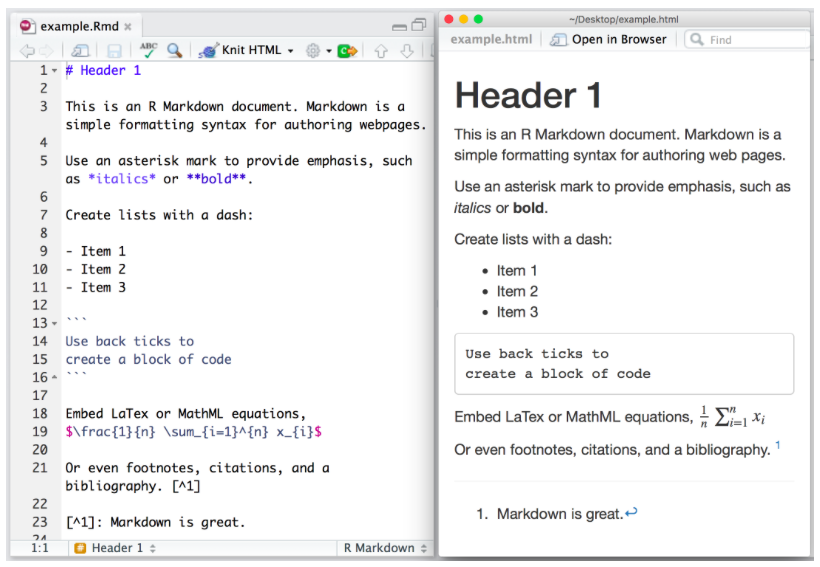
\includegraphics[scale=0.4]{figures/RmarkdownExample1.png}
\end{frame}
%----------
\begin{frame}
    \frametitle{Markdown}
    \begin{itemize}
        \item \underline{R Code Chunks} can be embedded with the native Markdown syntax for fenced code regions
        \item \underline{R expressions} inline by enclosing the expression within a single back-tick
        \item \underline{Inline text} \tiny\url{http://rmarkdown.rstudio.com/authoring_basics.html}
    \end{itemize}
\end{frame}
%-----------
\begin{frame}
    \frametitle{Markdown}
    \begin{center}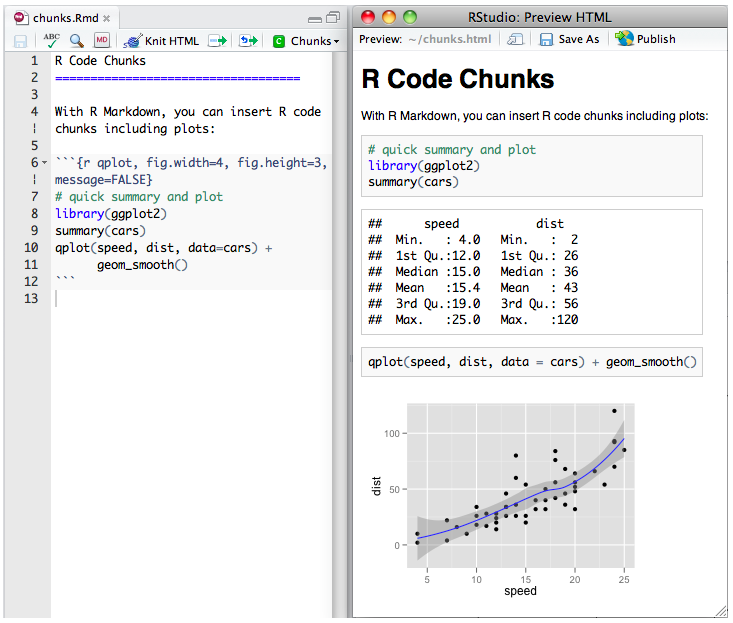
\includegraphics[scale=0.35]{figures/RmarkdownExample2.png}\end{center}
\end{frame}
%-----------
% Exercise 1 
%-----------
\begin{frame}
    \frametitle{Exercise 1}
    {\sc GOAL: create a default minimal document}
    \begin{itemize}
        \item Open RStudio
            \pause
        \item Select File $>$ New file $>$ R Markdown
            \pause
        \item Create an HTML document
    \end{itemize}
\end{frame}
%-----------------------
\begin{frame}
    \frametitle{Exercise 1}
    \begin{center}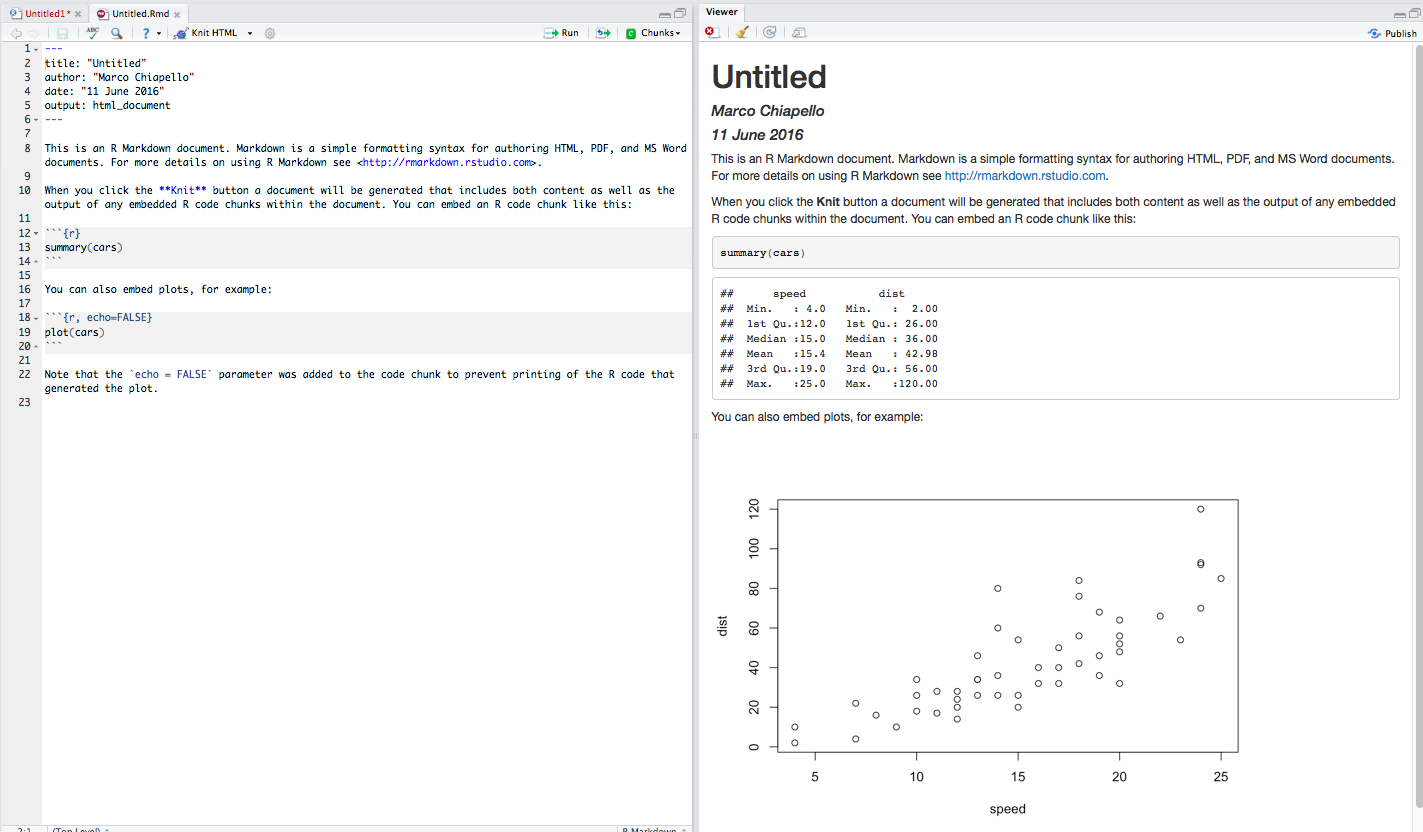
\includegraphics[scale=0.23]{figures/RmarkdownExample.png}\end{center}
\end{frame}
%-----------------------

%-------------
% Exercise 2
%-------------
\begin{frame}
    \frametitle{Exercise 2}
    {\sc GOAL: create a default minimal document}
    \begin{itemize}
        \item Create a pdf document
        \item Create a docx document
    \end{itemize}
\end{frame}

\end{document}

%------------------------
% Element explanation
%------------------------
\begin{frame}
    \frametitle{RMarkdown elements}
    \begin{itemize}
        \item Header
        \item Text
        \item Code chunks
    \end{itemize}
\end{frame}

\begin{frame}
    \frametitle{Header}
    -- Elements of the Header --
    -- Images --
    -- TOC --
\end{frame}

\begin{frame}
    \frametitle{Text}
    -- text styles --
    -- inline r code --
\end{frame}

\begin{frame}
    \frametitle{Code chunk}
    -- r options --
\end{frame}








